\section{Anhang}
\label{sec:Anhang}

\subsection{Bestimmung der kritschen Stromstärke $I_{\text{c}}$}
\label{sec:AnhangTc}

\begin{figure}[H]
    \centering
    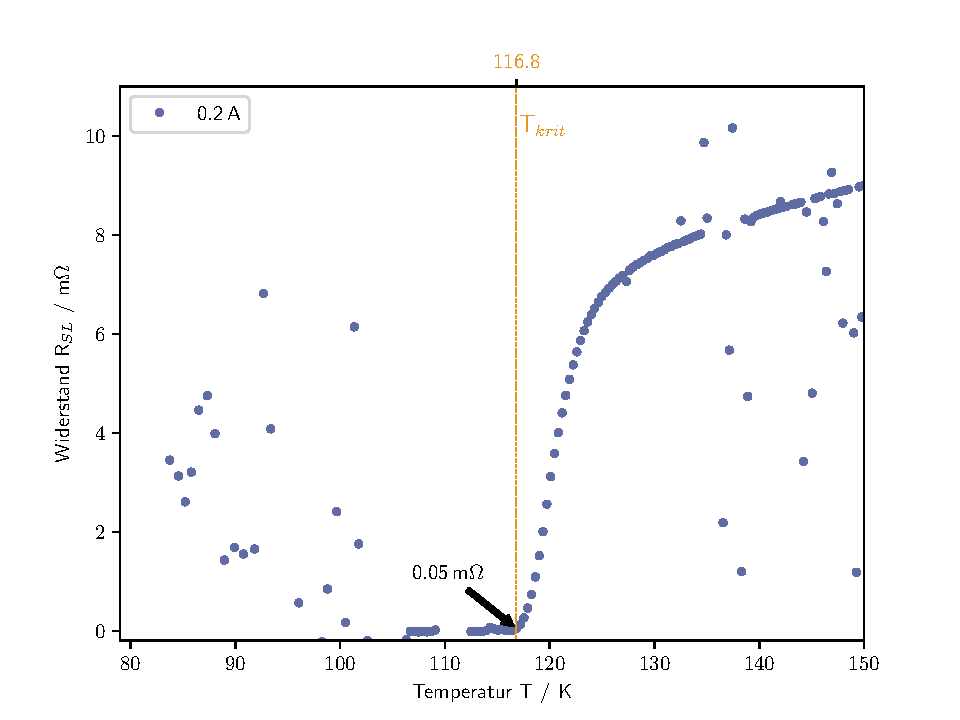
\includegraphics[width=0.8\textwidth]{Auswertung/I_krit_Pt/R_T_0.2A.pdf}
    \caption{Bestimmung der kritschen Temperatur des SL \#1 Supraleiter ohne Magnet
    anhand einer 4-Punkt-Messung. Die Temperatur $T$ wird mit einem Platin-Sensor
    ermittel, wobei der Widerstand $R_{\text{SL}}$ bei einem Strom $I$ von
    $\SI{0.2}{\ampere}$ gemessen wird.
		Die gelbe Markierung kennzeichnet die kritsche Temperatur	$T^{\text{4PM}}_{\text{c}}$.
		Es werden allen Messwerten einen systematischen Fehler von $\SI{\pm2}{\kelvin}$
		zugeschrieben.}
    \label{fig:Ic1.1}
\end{figure}

\begin{figure}[H]
    \centering
    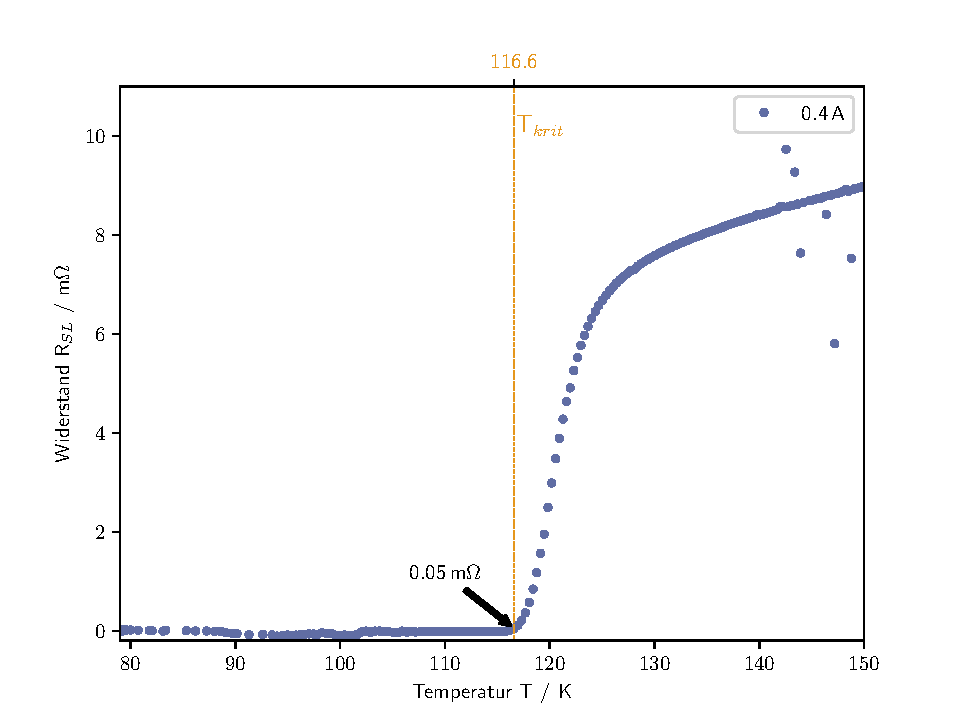
\includegraphics[width=0.8\textwidth]{Auswertung/I_krit_Pt/R_T_0.4A.pdf}
    \caption{Bestimmung der kritschen Temperatur des SL \#1 Supraleiter ohne Magnet
    anhand einer 4-Punkt-Messung. Die Temperatur $T$ wird mit einem Platin-Sensor
    ermittel, wobei der Widerstand $R_{\text{SL}}$ bei einem Strom $I$ von
    $\SI{0.4}{\ampere}$ gemessen wird.
		Die gelbe Markierung kennzeichnet die kritsche Temperatur	$T^{\text{4PM}}_{\text{c}}$.
		Es werden allen Messwerten einen systematischen Fehler von $\SI{\pm2}{\kelvin}$
		zugeschrieben.}
    \label{fig:Ic1.2}
\end{figure}

\begin{figure}[H]
    \centering
    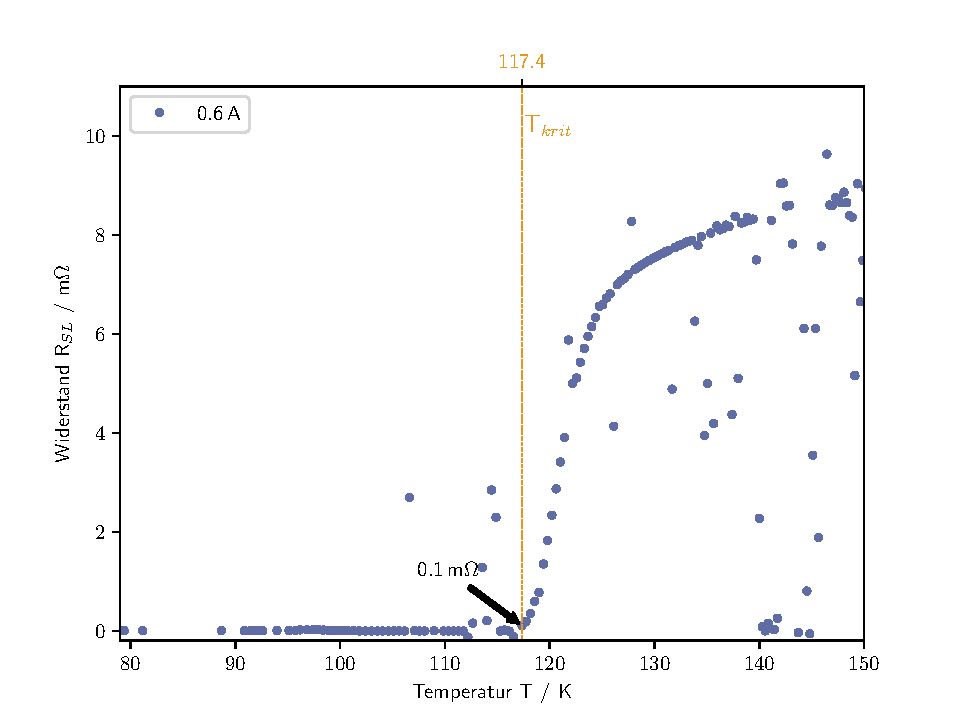
\includegraphics[width=0.8\textwidth]{Auswertung/I_krit_Pt/R_T_0.6A.pdf}
    \caption{Bestimmung der kritschen Temperatur des SL \#1 Supraleiter ohne Magnet
    anhand einer 4-Punkt-Messung. Die Temperatur $T$ wird mit einem Platin-Sensor
    ermittel, wobei der Widerstand $R_{\text{SL}}$ bei einem Strom $I$ von
    $\SI{0.6}{\ampere}$ gemessen wird.
		Die gelbe Markierung kennzeichnet die kritsche Temperatur	$T^{\text{4PM}}_{\text{c}}$.
		Es werden allen Messwerten einen systematischen Fehler von $\SI{\pm2}{\kelvin}$
		zugeschrieben.}
    \label{fig:Ic1.3}
\end{figure}

\begin{figure}[H]
    \centering
    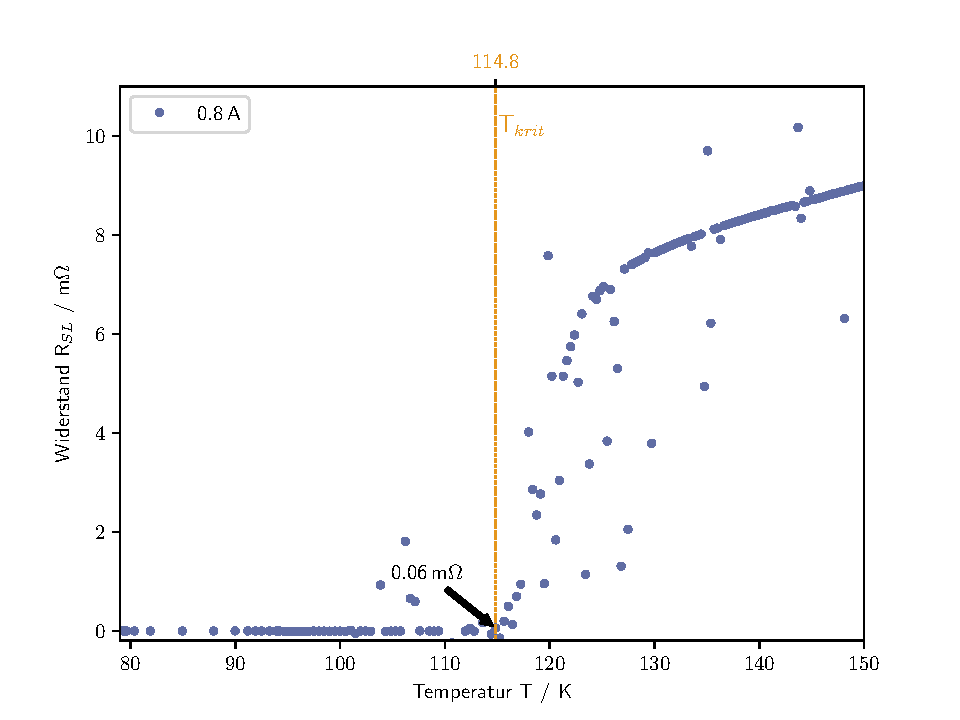
\includegraphics[width=0.8\textwidth]{Auswertung/I_krit_Pt/R_T_0.8A.pdf}
    \caption{Bestimmung der kritschen Temperatur des SL \#1 Supraleiter ohne Magnet
    anhand einer 4-Punkt-Messung. Die Temperatur $T$ wird mit einem Platin-Sensor
    ermittel, wobei der Widerstand $R_{\text{SL}}$ bei einem Strom $I$ von
    $\SI{0.8}{\ampere}$ gemessen wird.
		Die gelbe Markierung kennzeichnet die kritsche Temperatur	$T^{\text{4PM}}_{\text{c}}$.
		Es werden allen Messwerten einen systematischen Fehler von $\SI{\pm2}{\kelvin}$
		zugeschrieben.}
    \label{fig:Tc1.4}
\end{figure}

\begin{figure}[H]
    \centering
    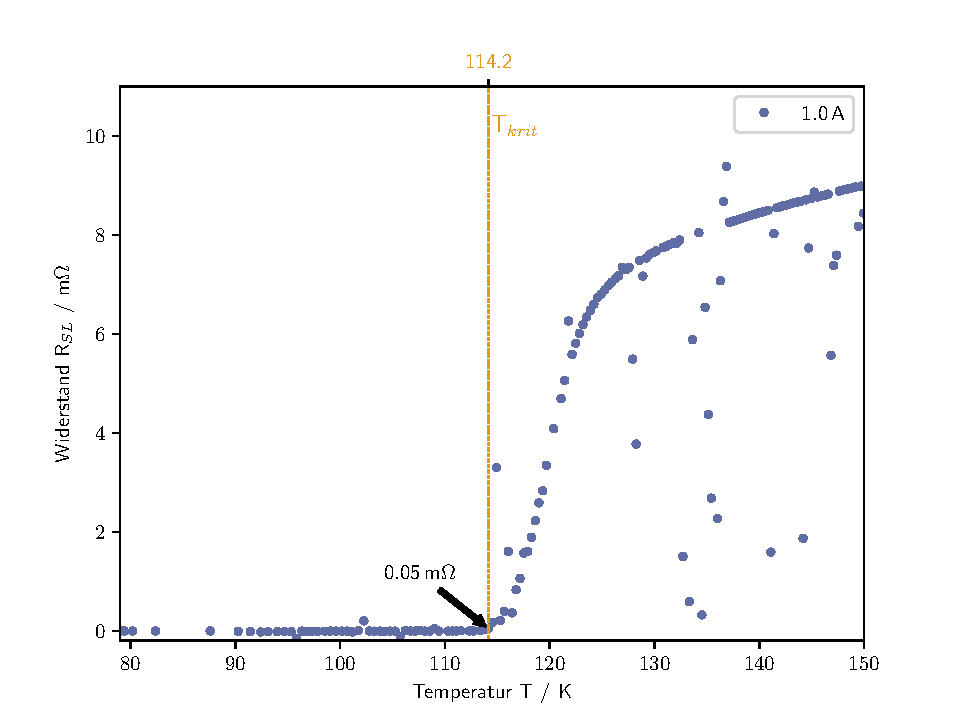
\includegraphics[width=0.8\textwidth]{Auswertung/I_krit_Pt/R_T_1.0A.pdf}
    \caption{Bestimmung der kritschen Temperatur des SL \#1 Supraleiter ohne Magnet
    anhand einer 4-Punkt-Messung. Die Temperatur $T$ wird mit einem Platin-Sensor
    ermittel, wobei der Widerstand $R_{\text{SL}}$ bei einem Strom $I$ von
    $\SI{1.0}{\ampere}$ gemessen wird.
		Die gelbe Markierung kennzeichnet die kritsche Temperatur	$T^{\text{4PM}}_{\text{c}}$.
		Es werden allen Messwerten einen systematischen Fehler von $\SI{\pm2}{\kelvin}$
		zugeschrieben.}
    \label{fig:Tc1.5}
\end{figure}

\begin{figure}[H]
    \centering
    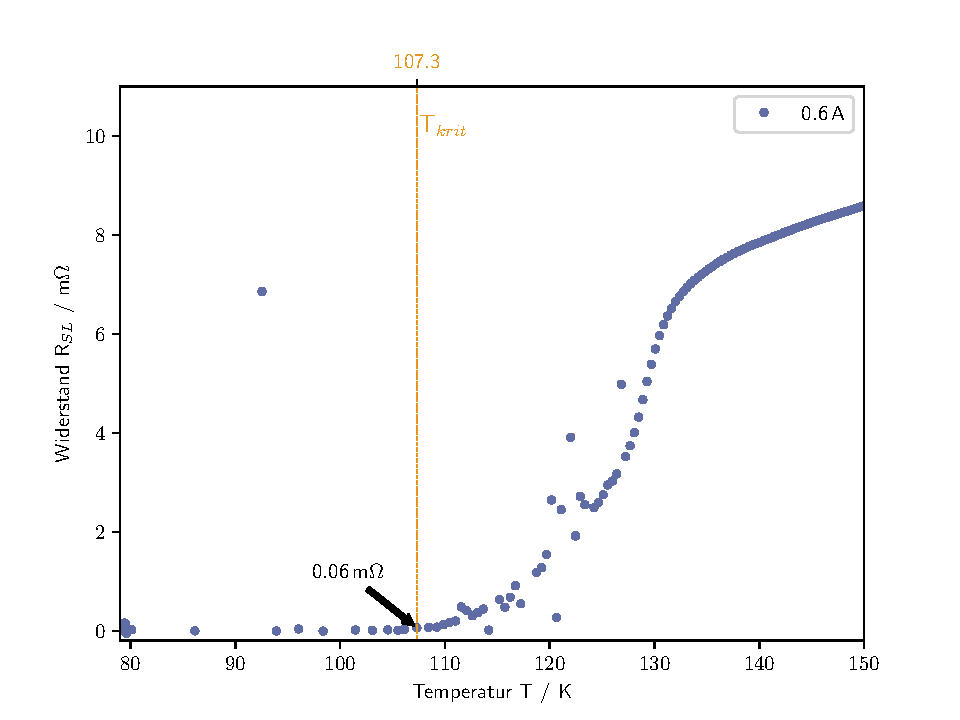
\includegraphics[width=0.8\textwidth]{Auswertung/I_krit_Pt_b/R_T_0.6A.pdf}
    \caption{Bestimmung der kritschen Temperatur des SL \#1 Supraleiter mit
    Störung des \#M3 Magnets anhand einer 4-Punkt-Messung. Die Temperatur $T$
    wird mit einem Platin-Sensor
    ermittel, wobei der Widerstand $R_{\text{SL}}$ bei einem Strom $I$ von
    $\SI{0.6}{\ampere}$ gemessen wird.
		Die gelbe Markierung kennzeichnet die kritsche Temperatur	$T^{\text{4PM}}_{\text{c}}$.
		Es werden allen Messwerten einen systematischen Fehler von $\SI{\pm2}{\kelvin}$
		zugeschrieben.}
    \label{fig:Tc2.1}
\end{figure}

\begin{figure}[H]
    \centering
    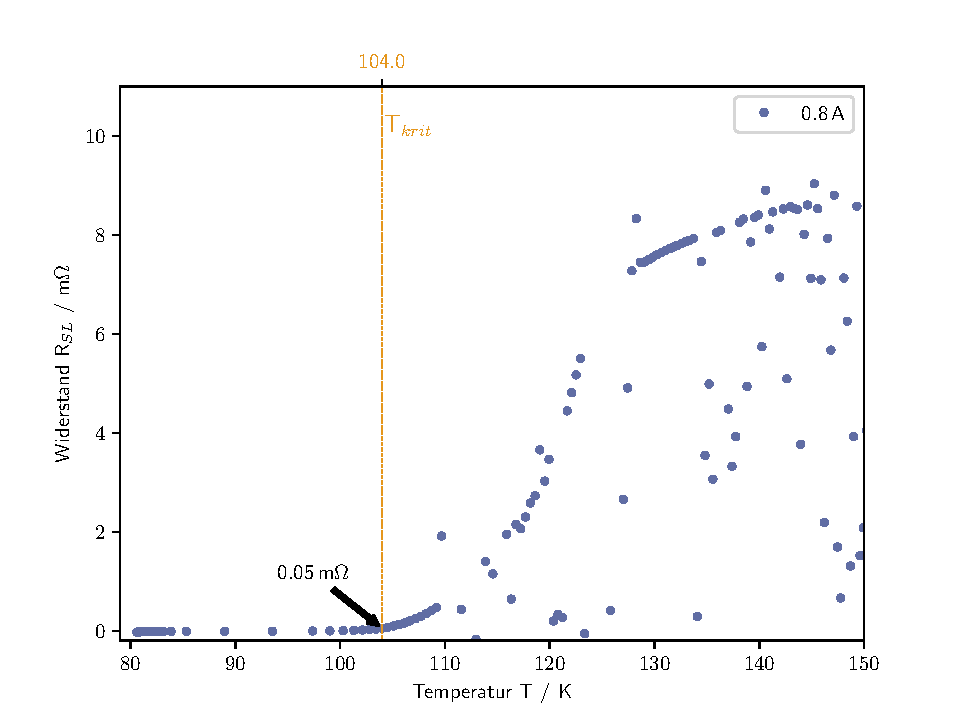
\includegraphics[width=0.8\textwidth]{Auswertung/I_krit_Pt_b/R_T_0.8A.pdf}
    \caption{Bestimmung der kritschen Temperatur des SL \#1 Supraleiter mit
    Störung des \#M3 Magnets anhand einer 4-Punkt-Messung. Die Temperatur $T$
    wird mit einem Platin-Sensor
    ermittel, wobei der Widerstand $R_{\text{SL}}$ bei einem Strom $I$ von
    $\SI{0.8}{\ampere}$ gemessen wird.
		Die gelbe Markierung kennzeichnet die kritsche Temperatur	$T^{\text{4PM}}_{\text{c}}$.
		Es werden allen Messwerten einen systematischen Fehler von $\SI{\pm2}{\kelvin}$
		zugeschrieben.}
    \label{fig:Tc2.2}
\end{figure}
